 \documentclass{report}
 
\usepackage[utf8]{inputenc} 
\usepackage[T1]{fontenc}      
\usepackage[top=2.0cm, bottom=3cm, left=3.0cm, right=3.0cm]{geometry}
\usepackage{graphicx}
\usepackage{wrapfig}
\usepackage{amsmath,esint }
\usepackage{amssymb}
\graphicspath{{figures/}{../figures}}

\newcommand*\dif{\mathop{}\!\mathrm{d}}
\newcommand*\diver{\mathop{}\!\mathrm{div}}
\newcommand*\grad{\mathop{}\!\mathrm{grad}}

\begin{document}

\section*{Lac gelé}

On s'intéresse à la glaciation d'un lac, et plus particulièrement de l'évolution au cours du temps de l'épaisseur de glace, notée $\xi(t)$, qui se forme à sa surface. L'interface entre l'atmosphère et la surface du lac se situe en $z=0$ et on considère qu'à $t=0$, le lac est encore libre de glace $\xi(t=0)=0$. On suppose que l'atmosphère est à la température constante $T_A=263$ K et que l'eau située sous la glace du lac est à la température de fusion $T_F$=273 K. 

\begin{figure}[h!]
\centering
  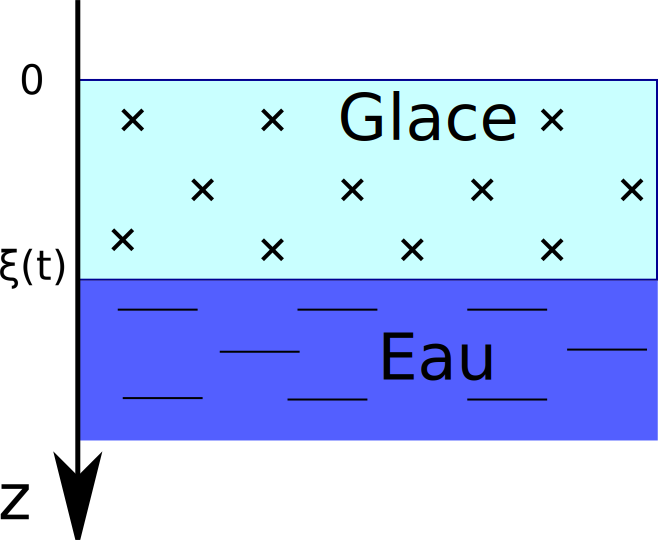
\includegraphics[width=0.4\textwidth]{diffusion_glace.pdf}
\end{figure}

Lors de la formation de la glace à l'interface $z=\xi(t)$, l'énergie thermique dégagée par la solidification de l'eau est évacuée à travers la glace jusqu'à l'atmosphère. On supposera que ce tranfert est instantané, ce qui revient à supposer que la glace a une capacité calorifique $c_g$ négligeable (hypothèse des régimes quasi-stationnaire).

D'autre part, les échanges thermiques entre l'atmosphère et la glace de la surface du lac sont modélisés par la loi de Newton : 
\begin{align*}
	\vec{j}_a=-h(T_0(t)-T_A)\vec{e}_z
\end{align*}
où $\vec{j}_a$ est la densité surfacique de flux thermique entre la glace et l'atmosphère, $T_0(t)$ est la température de la glace en $z=0$ et $h$ une constante égale à 42 W.m$^{-2}$.K$^{-1}$. Autrement dit, la surface du lac ne se thermalise pas instantanément avec l'atmosphère. 

On note par ailleurs $\rho_g=990$kg.m$^{-3}$ la masse volumique de la glace, $\lambda=2,1$ W.m$^{-1}$.K$^{-1}$ et la chaleur latente massique de fusion de l'eau $l_f=335$ kJ.kg$^{-1}$.

\begin{itemize}

	\item[$\ast$] Donner le profil de température $T(z,t)$ dans la glace en fonction de $T_0(t)$, $T_F$, $\xi(t)$ et $z$. 
	
	\item[$\ast$] En déduire la température de surface $T_0(t)$ en fonction de l'épaisseur de glace $\xi(t)$, et $h$, $T_A$, $T_F$, $\lambda$.
	
	\item[$\ast$] En faisant un bilan d'énergie sur le front de glaciation en $z=\xi(t)$, établir une relation entre $\xi(t)$ et $\dot{\xi}(t)$. En déduire l'équation différentielle suivante :
	\begin{align*}
		\left( 1+\frac{\xi(t)}{l_0}\right) \dot{\xi(t)}=v_0
	\end{align*}
	Préciser l'expression de $l_0$ et $v_0$.
	
	\item[$\ast$] Donner une estimation numérique de $l_0$ et de $v_0$. En déduire un temps caractéristique $\tau_0$ dont on donnera aussi une estimation numérique. %L'approximation des régimes quasi-stationnaire est-elle valable ? 
	
	\item[$\ast$] Déterminer l'évolution de $\xi(t)$ puis de $T_0(t)$ et donner l'allure de leur courbe. Combien de temps faut-il pour que 5 cm de glace ne se forment ?
	
\end{itemize}	
	
\newpage

\section*{Transfert thermique et entropie}

On considère une barre métallique conductrice de section $S$, de longueur $L$, de résistivité électrique $\rho$ et de conductivité thermique $\lambda$. On suppose que ces extrémités sont maintenues aux températures $T_1$ et $T_2$ grâce à des thermostats, et que les parois extérieures sont calorifugées sur toute la longueur du barreau. En régime permanent, elle est parcourue par un courant $I$.

\begin{itemize}

	\item[$\triangleright$] Déterminer le profil de température $T(x)$ dans la barre, où $x$ est l'abcsisse le long de celui-ci.
	
	\item[$\triangleright$] A quelle condition la température passe par un maximum ? 
	
	\item[$\triangleright$] Calculer l'entropie $s_c$ créée par unité de temps et de volume dans la barre à une abscisse $x$. Commenter.

\end{itemize}

On coupe désormais le courant dans la barre ($I=0$), puis une fois le nouveau régime permanent établi, on l'isole totalement des thermostats.

\begin{itemize}
		
	\item[$\triangleright$] Obtenir le nouveau profil de température juste avant que les deux thermostats soient retirés de la barre.
	
	\item[$\triangleright$] Une fois les thermostats enlevés, quelle sera la température finale $T_\infty$ de la barre après avoir suffisament attendu ? En déduire la variation d'entropie de la barre.
	
\end{itemize}

\newpage

\section*{Combustion d'une poutre de bois}

On considère une poutre en bois homogène de section carrée $S$ et de longueur $L$ rentrant en combustion à l'instant $t=0$ en $x=0$. On cherche à comprendre la progression de la combustion le long de la poutre, en supposant que celle-ci est uniquement dûe à la diffusion de la chaleur dans le bois. 
A l'instant $t$, on distingue la combustion en 3 zones distinctes :
\begin{itemize}
	\item[-] une zone brulée, située entre $x=0$ et $x_1(t)$, à la température uniforme $T_c=720$ K dite de combustion ;
	\item[-] une zone dans laquelle s'effectue la combustion, située entre $x_1(t)$ et $x_2(t)$, dégageant une puissance thermique massique $P_c=4,0\times10^3$ W.kg$^{-1}$ ;
	\item[-] et une zone inaltérée, où le bois est encore intact, située entre $x_2(t)$ et $L$
\end{itemize}
La température $T(x,t)$ dans la zone en combustion et celle de la zone inaltérée augmentent par diffusion au cours du temps jusqu’à atteindre les températures de combustion $T_c$ et d’inflammation du bois $T_i=$520 K, conduisant à l’avancement des frontières $x_1(t)$ et $x_2(t)$ au cours du temps. Ainsi, tant que la poutre n’a pas fini de bruler, on a toujours $T(x_1(t),t)=T_c$ et $T(x_2(t),t)=T_i$. D'autre part, loin du front de combustion $x_1(t)$, la température de la poutre est $T_\infty=320$ K.

\begin{figure}[h!]
\centering
  \includegraphics[width=0.9\textwidth]{poutre.png}
\end{figure}

On considère enfin que le bois brulé, en combustion ou inaltéré est un même matériau homogène, de capacité calorfique massique à pression constante $c_p=2,0\times10^3$ J.K$^{-1}$.kg$^{-1}$, de diffusivité thermique $D=1,0\times10^{-7}$m$^2$.s$^{-1}$ et de masse volumique $\mu=850$kg.m$^{-3}$.

\begin{itemize}

	\item[$\Join$] En effectuant un bilan d'enthalpie sur un élément de bois compris entre $x$ et $x+dx$ dans la zone en combustion, montrer que la température vérifie l'équation suivante :
	\begin{align*}
		\frac{\partial T}{\partial t}=D\frac{\partial^2 T}{\partial x^2} + \kappa
	\end{align*}
	Préciser l'expression de $\kappa$.
	\item[$\Join$] De même, trouver l'équation vérifiée par $T$ dans la zone brulée et inaltérée. 

\end{itemize}

On se propose de résoudre les équations précédentes sous forme d’une onde se propageant dans la poutre. On pose $u=x-ct$ où $c$ est une constante positive et on effectue le changement de variable $T(x,t)=\theta(u)$.

\begin{itemize}

	\item[$\Join$] Que représente physiquement $c$ ? 
	\item[$\Join$] Déterminer les équations différentielles régissant la fonction $\theta(u)$ dans les trois zones, puis montrer que les solutions peuvent s'écrire :
	\begin{align*}
		\left\{
    \begin{array}{ll}
        \theta(u)=a_1 & \mbox{pour } u<u_1 \\
       \theta(u)=a_2 + b_2\exp\left( -\frac{c}{D}u\right)  - \frac{\kappa}{c}u & \mbox{pour } u_1<u<u_2 \\
       \theta(u)=a_3 + b_3\exp\left( -\frac{c}{D}u\right)  u_2<u
    \end{array}
\right.
	\end{align*}
	\item[$\Join$] Déterminer les expressions de $a_1$ et de $a_3$ avec les données de l'énoncé, puis expliciter les conditions permettant de trouver $a_2$, $b_2$ et $b_3$ (on ne cherchera pas à obtenir leur expression).
	\item[$\Join$] Tracer l'allure de la courbe $\theta(u)$. Commenter. 
	
\end{itemize}

\newpage	

\section*{Température dans une planète naine}

On s'intéresse au profil de température au sein d'une planête naine, faisant 100 km de rayon. On suppose qu'elle est intégralement constitué de roches proches du granit (conductivité thermique $\lambda = 3,5$ W.m$^{-1}$.K$^{-1}$, masse volumique $\mu=2700$ kg.m$^{-3}$ et capacité calorifique massique $c_p=790$ J.K$^{-1}$.s$^{-1}$), sans activité géologique, c'est-à-dire que l'astre est figé, sans convection possible à l'intérieur. Il existe de surcroit une activité radioactive dûe à la présence de thorium 232($^{232}$Th, masse molaire $M=232$ g.mol$^{-1}$) uniformément réparti dans le volume, dont la désintégration dégage une énergie $\varepsilon=5,6\times10^{-12}$ J, avec une demi-vie de $\tau=14\times10^{10}$ années.

\begin{itemize}

	\item[$\circledcirc$] La concentration massique de thorium étant de l'ordre de 10 ppm, estimer la puissance volumique $P_r$ due à la désintégration du thorium.
	
	\item[$\circledcirc$] Le problème étant supposé à symétrie sphérique, effectuer un bilan d'enthalpie entre deux couches adjacentes de roche de rayon $r$ et $r+dr$ et montrer que la température vérifie l'équation suivante :
	\begin{align*}
		\frac{\partial T}{\partial t}=\frac{D}{r^2}\frac{\partial }{\partial r}\left( r^2\frac{\partial T}{\partial r}\right)  + \kappa		
	\end{align*}
Préciser l'expression de $\kappa$ et de $D$.

	\item[$\circledcirc$] Montrer que l'on peut se placer dans le régime quasi stationnaire $T(r,t)\simeq T(r)$, c'est-à-dire que l'activité nucléaire varie très lentement par rapport au temps caractéristique $\tau_d$ de diffusion thermique. 
	
	\item[$\circledcirc$] Exprimer l'expression du champ de température $T(r)$ à l'aide de deux constantes d'intégration. Montrer que l'une d'entre elle est nécessairement nulle.
	
\end{itemize}

	 La planète perd de l'énergie thermique par rayonnement, qui part dans l'espace depuis sa surface. La puissance thermique associée à ce rayonnement suit la loi de Stefan-Boltzmann $\phi=\sigma T_s^4$, où $\phi$ est la puissance rayonnée par unité de surface à la surface de la planète, $\sigma=5,67\times10^{-8}$ W.m$^{-2}$.K$^{-4}$ une constante et $T_s$ la température à la surface de l'astre.

\begin{itemize}

	 \item[$\circledcirc$] En utilisant la loi de Stefan-Boltzmann, déterminer la seconde constante d'intégration et donner l'expression de la température $T(r)$.
	 
	 \item[$\circledcirc$] Donner la valeur de la température au centre de la planète et à la surface.

\end{itemize}	

On donne, pour les coordonnées sphériques : $\vec{\mathrm{grad}} f\cdot \vec{e}_r = \frac{\partial f}{\partial r}$

\newpage

\section*{Une tente au soleil}

Un campeur se trouve allongé dans sa tente canadienne. Le soleil se lève et éclaire une des faces de la tente, mais pas l'autre. Pour se refroidir, est-ce une bonne idée pour notre campeur de se mettre en position assise ? 
	
\vspace*{2cm}	
	
\begin{figure}[h!]
\centering
  \includegraphics[width=0.7\textwidth]{tente.jpg}
\end{figure}

\newpage	

\section*{Diffusion de particules dans un récipent en rotation}

Des particules de masse $m$, de rayon $a$ et de masse volumique $\rho_p$ sont en suspension dans un solvant de masse volumique $\rho_s$ et de viscosité $\eta$, contenu dans un récipent. Elles subissent par ailleurs une force de frottement fluide $-6\pi\eta a\vec{v}$ lorsqu'elles sont en mouvement à la vitesse moyenne $\vec{v}$. Le coefficient de diffusion de ces particules dans le solvant est noté $D$.

\subsubsection*{Cas statique : sédimentation}

\begin{itemize}
	
	\item[$\odot$] En régime permanent, établir la vitesse moyenne d'une particule isolée qui sédimente, soumise à son poids, à la poussée d'Archimède et à la force de frottement fluide.	On introduira la masse effective $m^*=m\left( 1-\frac{\rho_s}{\rho_p}\right) $. Quel est le flux de particules $\vec{j}_s$ associé à cette sédimentation ? 
	
	\item[$\odot$] Ce flux de sédimentation est compensée par le phénomène de diffusion. Expliquer le phénomène. 
	
	\item[$\odot$] En faisant un bilan de particules sur un volume élémentaire, montrer que la concentration de particule $c$ est reliée à $\vec{j}_s$ et au flux de particule $\vec{j}_D$ dû à la diffusion par la relation suivante :
	\begin{align*}
		\frac{\partial c}{\partial t}=-\diver(\vec{j}_D+\vec{j}_s)
	\end{align*}
	
	\item[$\odot$] En déduire la concentration de particule $c(z)$ dans le récipient en régime permanent.
	
\end{itemize}

\subsubsection*{Cas dynamique}

On fait tourner désormais le récipient à une vitesse angulaire $\omega$, soumettant les particules à une force centrifuge $\vec{f}_r=m\omega^2r\vec{e}_r$. On néglige désormais le poids des particules.

\begin{itemize}

	\item[$\odot$] Montrer que la concentration en particules vérifient l'équation suivante :
	\begin{align*}
		\frac{\partial c}{\partial t}=\frac{1}{r}\frac{\partial }{\partial r}\left(r\left(D\frac{\partial c}{\partial r} -sr\omega^2c(r) \right) \right)
	\end{align*}
	Préciser l'expression de $s$.
	
	\item[$\odot$] En déduire la concentration de particules en régime permanent. 

\end{itemize}

\newpage

\section*{Diffusion à contre-courant}

Dans un tuyau de section $S$ circule un solvant à la vitesse $-v_0\vec{e}_x$, où $x$ est l'axe le long du tuyau. En $x=0$, on injecte à travers une petite ouverture un colorant dans le tuyau, avec un débit molaire $n^*$. On suppose que le colorant s'homogénéise immédiatement sur toute la section $S$ du tuyau dès son injection en $x=0$. On remarque que, en plus de s'évacuer avec le solvant vers les $x$ négatifs, le colorant remonte à contre-courant sur une longueur caractéristique $L$. Le coefficient de diffusion du colorant dans le solvant est noté $D$.

\begin{itemize}

	\item[$\spadesuit$] Montrer que la concentration $c$ de particules de colorant en aval de l'écoulement $(x<0$) ne dépend de $x$ et s'écrit $c=\frac{N_A n^*}{v_0S}$, en notant $N_A$ le nombre d'Avogadro. En déduire le flux de particule associé $\vec{j}_c$.
	
	\item[$\spadesuit$] Pourquoi la concentration $c$ va dépendre de $x$ en amont de l'écoulement $(x<0$) ? Quel est le flux de particule $\vec{j}_c(x)$ associé ?
	
	\item[$\spadesuit$] En déduire une équation différentielle sur $c(x)$. La résoudre, et en déduire la longueur $L$ de remontée à contre-courant.

\end{itemize}

\newpage

\section*{Evaporation de l'éther}

Un tube à essai de section $S$ est rempli d'éther (masse volumique $\mu=626$ kg.m$^{-1}$, masse molaire $M=74$ g.mol$^{-1}$), à une distance $h(t)$ du bord. L'éther étant un liquide très volatile , il s'évapore progressivement de sorte à ce que la hauteur $h$ augmente. A la surface de l'éther, il y a un équilibre vapeur/liquide à la pression de vapeur saturante de l'éther $P_{sat}=0,583$ mbar (à une température $T=293K$ que l'on supposera fixe). Au bord du tube, l'éther est vite dilué dans l'air ambiant et sa concentration est donc nulle. Sa diffusivité dans l'air est notée $D=1,5\times10^{-5}$m$^2$.s$^{-1}$.

\begin{figure}[h!]
\centering
  \includegraphics[width=0.2\textwidth]{ether2.pdf}
\end{figure}

\begin{itemize}

	\item[$\blacktriangle$] En notant $c(x)$ la concentration molaire en vapeur d'éther dans le tube entre $0$ et $h(t)$, retrouver l'équation de diffusion sur $c(x)$ en supposant la loi de Fick vérifiée.
	
	\item[$\blacktriangle$] En déduire la concentration de vapeur d'éther $c(x)$ dans le tube en fonction de $x$, $h(t)$, $P_{sat}$, $R$ et $T$. On supposera qu'on est en régime quasi-stationnaire.
	
	\item[$\blacktriangle$] Quelle quantité d'éther $dN$ est évaporée entre $t$ et $t+dt$ ? 
	
	\item[$\blacktriangle$] En déduire l'équation différentielle suivante :
	\begin{align*}
		h\dot{h}=C		
	\end{align*}
	où $C$ est une constante que l'on précisera.
	
	\item[$\blacktriangle$] En déduire un ordre de grandeur du temps d'évaporation de l'éther.

\end{itemize}

\end{document}